\section{Methodology}

\subsection{Framework Overview}
GenAU couples two jointly-trained pathways (Figure~\ref{fig:Model-Arch}): (1) a \emph{text} pathway that generates text conversation and (2) a \emph{visual grounding} pathway that uses the hidden states of the generated \texttt{[SEG\_normal]}/\texttt{[SEG\_defect]} tokens as language-grounded anchors, aligned with multi-scale visual features to produce pixel-level anomaly maps; the image-level score fuses the map maximum with the decoder's normal/defect decision.
\begin{figure*}[t]
  \centering
  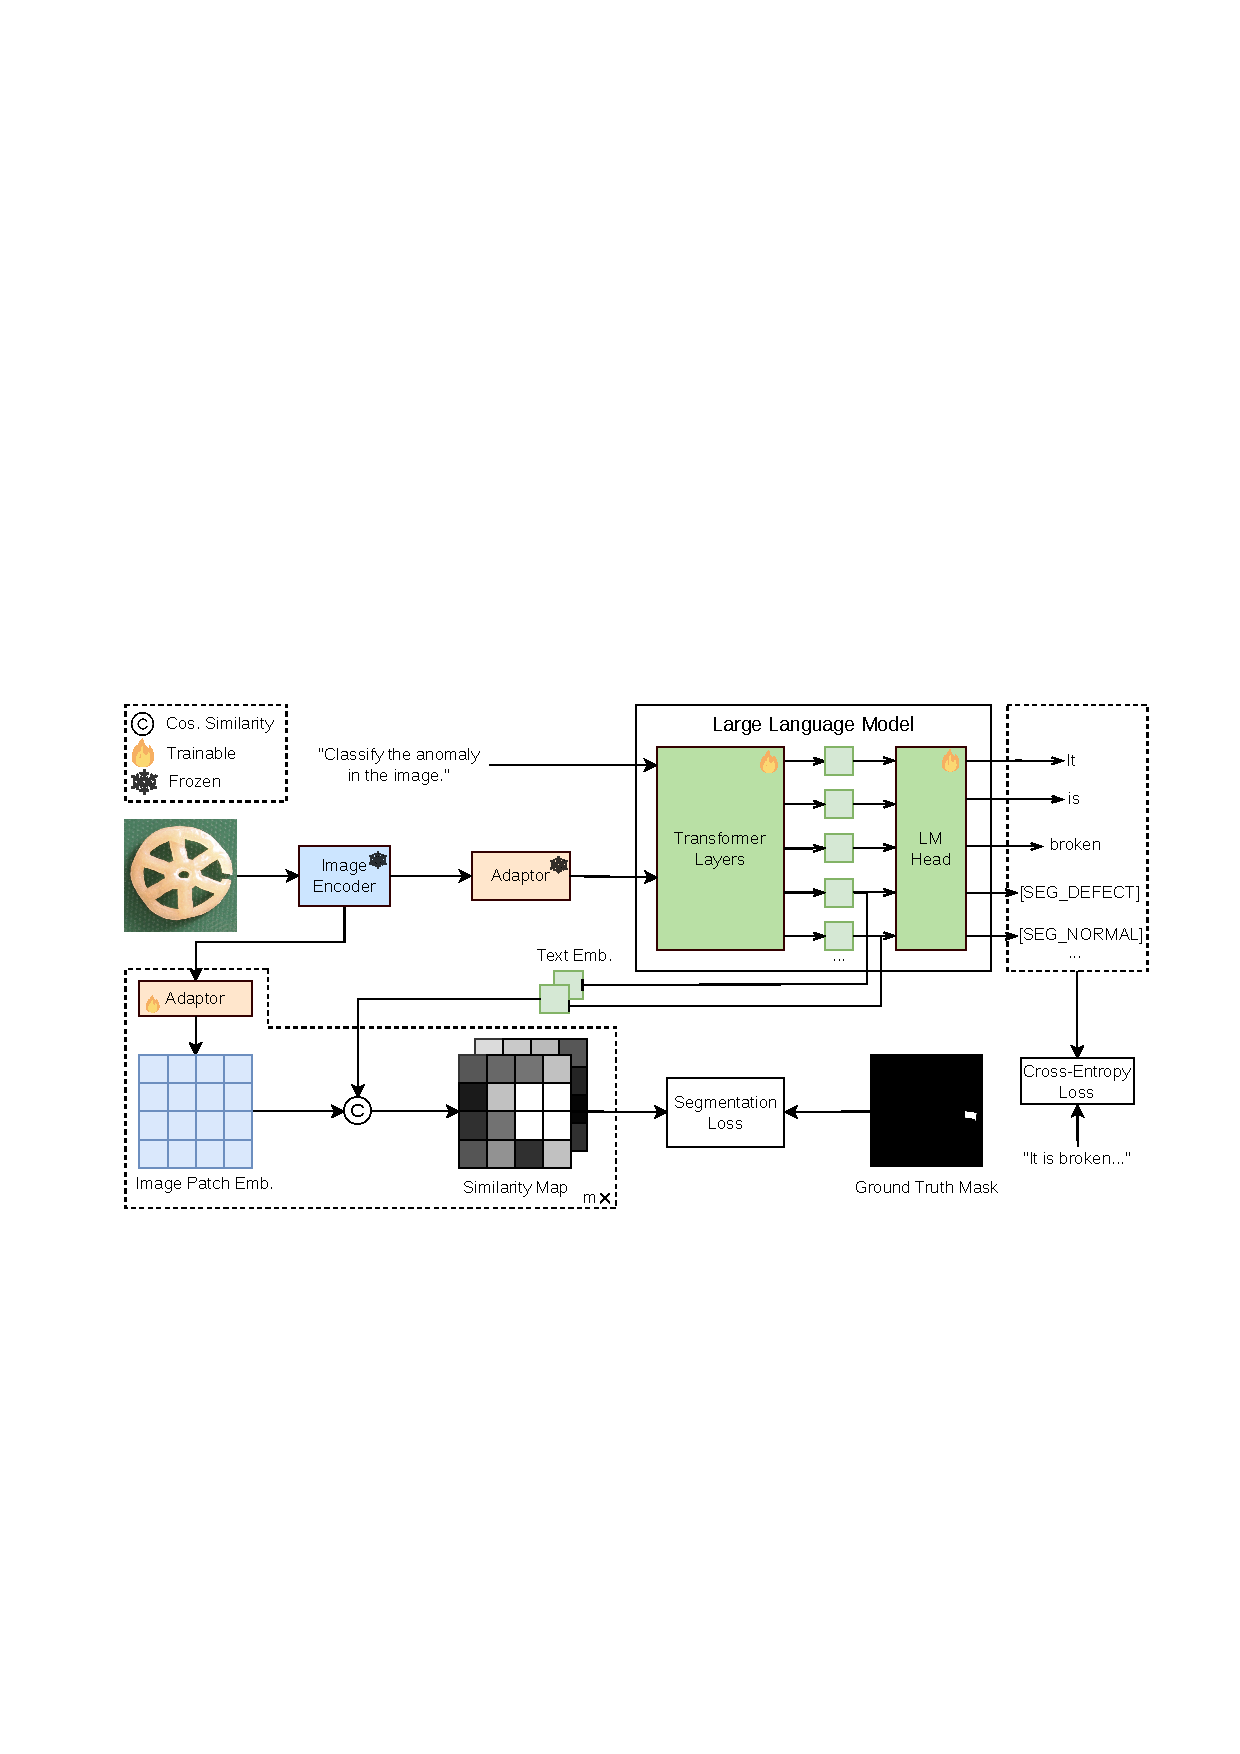
\includegraphics[width=1.0\textwidth]{imgs/GenAU_Arch_final.pdf}
  \caption[Overview of the training phase of GenAU.]{Overview of GenAU training. A frozen image encoder feeds the LLM, which generates the defect type and the \texttt{[SEG]} tokens (cross-entropy). In parallel, per-layer projections of the intermediate patch features are matched against the \texttt{[SEG]} hidden states to form the similarity map (focal + Tversky + Dice).}
   \label{fig:Model-Arch}
\end{figure*}


\subsection{Anomaly Segmentation}
\label{subsec:seg}
% The segmentation pathway computes the similarity between image and text features, inspired by prior work such as AnomalyCLIP~\cite{zhou2024anomalyclip}, MultiADS~\cite{sadikaj2025multiadsdefectawaresupervisionmultitype}, and APRIL-GAN~\cite{chen2023zero}. An image patch is classified as anomalous if its corresponding visual embedding exhibits high similarity to an anomaly-specific text embedding.
% Unlike CLIP-based models, instruction-following VLMs typically lack an explicit text encoder, making direct prompt embedding infeasible. Instead, GenAU leverages the LLM’s generative capacity to produce text embeddings conditioned jointly on the input image $\mathbf{X}_v$ and instruction $\mathbf{H}_q$. This approach allows the resulting embeddings to be contextually grounded in both the visual and linguistic input, rather than being static representations of predefined prompts. Consequently, the embeddings better capture fine-grained semantic alignment between the visual content and defect-specific textual concepts. Inspired by Lai et al.~\cite{lai2024lisareasoningsegmentationlarge}, two special tokens, \texttt{[SEG\_defect]} and \texttt{[SEG\_normal]}, are introduced into the model vocabulary. These tokens act as semantic anchors for anomalous and normal regions, respectively, and are generated immediately following the predicted defect type.
% Since the model is autoregressive, each segmentation token is conditioned on the preceding defect token, allowing the attention mechanism to encode spatial-semantic dependencies useful for segmentation. The latent representations of these tokens, extracted from the final hidden state of the LLM, serve as the anchors $\mathbf{z}^t \in \mathbb{R}^{N_z}$ for the normal and defect states.
% Each input image $\mathbf{X}_v$ is simultaneously processed by the vision encoder, which extracts patch-wise features from $m$ intermediate stages, as in APRIL-GAN~\cite{chen2023zero}. For stage $i$, the resulting feature map is $\mathbf{e}_i^p \in \mathbb{R}^{h \times w}$, where $h \times w$ denotes spatial resolution. To align the differing embedding spaces of the vision and language modalities, a set of stage-specific linear projection layers is introduced. Each layer maps its corresponding visual features into the LLM’s embedding space, producing projected features $\mathbf{z}_i^p \in \mathbb{R}^{h \times w}$.
% After projection, cosine similarity is computed between each patch embedding and both the normal and defect text embeddings to produce stage-wise similarity maps:
% $\mathbf{S}_i = \frac{\mathbf{z}_i^p}{\|\mathbf{z}_i^p\|} \cdot \frac{\mathbf{z}_i^t}{\|\mathbf{z}_i^t\|},$
% where $\mathbf{S}_i \in \mathbb{R}^{h \times w \times 2}$, and the two channels correspond to the similarity with the normal and defect descriptors, respectively.
% The similarity maps are upsampled to the input resolution and normalized across channels via softmax, yielding a per-pixel anomaly probability map. A higher activation in the anomaly channel indicates stronger confidence of defect presence.
GenAU performs anomaly localization by grounding visual features with the hidden states of generated segmentation tokens. Given an image $\mathbf{X}_v$ and an instruction $\mathbf{X}_q$, the autoregressive decoder generates a structured response containing the special tokens \texttt{[SEG\_normal]} and \texttt{[SEG\_defect]}. Let $\mathbf{h}_{\mathrm{normal}}, \mathbf{h}_{\mathrm{defect}}\in\mathbb{R}^{D}$ denote their final-layer decoder hidden states. These two vectors serve as language-grounded anchors for the normal and defective states:
Here, language-grounded denotes conditioning on the image, instruction, and preceding response through the decoder; it is not a claim that linguistic semantics alone explain the localization gain.
\begin{equation}
    \mathbf{T}
    =
    [\mathbf{h}_{\mathrm{normal}}, \mathbf{h}_{\mathrm{defect}}]
    \in \mathbb{R}^{2\times D}.
\end{equation}

The input image is processed by the frozen vision encoder to obtain multi-scale patch features from intermediate and final stages,
\(\{\mathbf{V}_i\}_{i=1}^{m}\), where
\(\mathbf{V}_i\in\mathbb{R}^{H_iW_i\times C_i}\) denotes the patch features from the \(i\)-th stage. Since the visual features and decoder hidden states lie in different representation spaces, each stage is equipped with its own \emph{linear} projection layer
\(\phi_i:\mathbb{R}^{C_i}\rightarrow\mathbb{R}^{D}\), producing
\begin{equation}
    \mathbf{Z}_i
    =
    \phi_i(\mathbf{V}_i)
    \in
    \mathbb{R}^{H_iW_i\times D}.
\end{equation}

For each stage, we compute cosine-similarity logits between every projected patch feature and the two segmentation-token anchors:
\begin{equation}
    \mathbf{S}_i
    =
    \gamma
    \cdot
    \frac{\mathbf{Z}_i}{\|\mathbf{Z}_i\|_2}
    \left(
    \frac{\mathbf{T}}{\|\mathbf{T}\|_2}
    \right)^{\top},
    \qquad
    \mathbf{S}_i\in\mathbb{R}^{H_iW_i\times 2},
\end{equation}
where \(\gamma\) is a fixed temperature scale. The two channels of \(\mathbf{S}_i\) correspond to the normal and defect scores. After reshaping \(\mathbf{S}_i\) to spatial resolution \(H_i\times W_i\), the maps are upsampled to the target mask resolution and normalized with a channel-wise softmax. The defect-channel probability gives the pixel-level anomaly map:
\begin{equation}
    \mathbf{A}_i
    =
    \mathrm{Softmax}(\mathrm{UP}(\mathbf{S}_i))_{[\mathrm{defect}]}
    \in
    [0,1]^{H\times W}.
\end{equation}
The stage-wise maps are aggregated by summation across the $m$ stages to form the final anomaly map $\mathbf{A}$, where higher values indicate a higher probability that the corresponding pixels belong to defective regions.

\paragraph{AnyRes high-resolution readout.}
The backbone encodes high-resolution inputs with an AnyRes scheme that, besides a global low-resolution view, splits the image into a grid of higher-resolution tiles. Applying the readout above to the global view alone yields a coarse low-resolution grid. To recover fine spatial detail, GenAU reassembles the patch features of the AnyRes tiles into a single high-resolution feature grid and computes the same anchor-grounded similarity maps on it. At inference, the high-resolution map $\mathbf{A}^{\mathrm{hi}}$ and the global-view map $\mathbf{A}^{\mathrm{g}}$ are fused per stage as $\mathbf{A}=(1-\beta)\,\mathbf{A}^{\mathrm{g}}+\beta\,\mathbf{A}^{\mathrm{hi}}$ with a fixed weight $\beta$. This high-resolution readout is used for all reported segmentation results.

\subsection{Image-level Anomaly Scoring}
Building on the segmentation map above, GenAU computes the image-level anomaly score without training a separate image-level classifier. Let $\mathbf{A}$ denote the final anomaly map of Section~\ref{subsec:seg} (the stage-aggregated defect response). The image-level anomaly score is its spatial maximum,
\begin{equation}
    s_{\mathrm{img}}
    =
    \max_{(u,v)}\mathbf{A}(u,v),
\end{equation}
where a larger $s_{\mathrm{img}}$ indicates a higher probability that the image contains an anomaly. This score introduces no additional trainable parameters and is obtained entirely from the language-grounded segmentation readout.

\paragraph{Fused image-level score.}
The map maximum $s_{\mathrm{img}}$ is a purely visual readout. Because the decoder additionally emits an explicit normal/defect decision, the image-level score we report is
\begin{equation}
    s_{\mathrm{fused}}
    =
    \tfrac{1}{2}\,\tilde{s}_{\mathrm{img}}
    +
    \tfrac{1}{2}\,\tilde{\ell}_{\mathrm{nd}},
\end{equation}
where $\ell_{\mathrm{nd}}$ is the decoder's normal/defect (yes/no) log-odds averaged over eight phrasings of the detection question (the question templates of the VisA and MPDD benchmarks; the image prefix is encoded once and reused), and the visual score $\tilde{s}_{\mathrm{img}}$ and $\tilde{\ell}_{\mathrm{nd}}$ are each standardized by a frozen calibration estimated once on MVTec (Appendix~\ref{app:impl}); no target-domain labels are used. Unless stated otherwise, all reported image-level results use $s_{\mathrm{fused}}$.



\subsection{Textual Reasoning and Multi-Type Anomaly Detection}
%We leverage the general-purpose visual understanding of large VLMs and adapt them for industrial anomaly detection through targeted fine-tuning on a single-label classification task. 
% The model is trained to predict the specific defect type present in an image, enabling it to capture subtle, domain-specific visual cues such as surface imperfections, texture irregularities, and localized damage that are critical for industrial inspection. 
For conditional defect-type recognition, GenAU receives a known-anomalous target image $\mathbf{X}_v$ and an instruction listing its object's coarse candidate labels $C_{\mathrm{target}}(o)$. It generates a response $\mathbf{X}_a$; a deterministic parser $\pi(\cdot)$ selects one label $\hat{y}'\in C_{\mathrm{target}}(o)$, or an unmatched sentinel counted as an error (Appendix~\ref{app:eval}). Compound labels represent combinations as one class, rather than independent per-type predictions.
% Thus, instead of learning a fixed classifier over $C_{\mathrm{train}}$, GenAU formulates multi-type anomaly detection as constrained conditional generation over $C_{\mathrm{target}}$, preserving language reasoning while producing domain-specific, machine-readable predictions.

\subsection{Training Objective}

GenAU is optimized with a joint objective that supervises textual reasoning and pixel-level anomaly segmentation. For each training sample, the model receives an image $\mathbf{X}_v$ and an instruction $\mathbf{X}_q$, and is trained to generate a structured response $\mathbf{X}_a=(a_1,\ldots,a_T)$ containing the predicted defect type and the grounding tokens \texttt{[SEG\_normal]} and \texttt{[SEG\_defect]}. The overall objective is
\begin{equation}
    \mathcal{L}
    =
    \mathcal{L}_{\mathrm{txt}}
    +
    \lambda_{\mathrm{seg}}\mathcal{L}_{\mathrm{seg}},
    \label{eq:overall-loss}
\end{equation}
where $\lambda_{\mathrm{seg}}$ balances the language-modeling and pixel-level supervision terms. The image-level anomaly score is computed at inference from the segmentation map and the decoder's yes/no log-odds (Sec.~\ref{subsec:seg}) and thus requires no dedicated training term.

\paragraph{Text generation loss.}
The textual reasoning objective is the standard autoregressive cross-entropy loss over the target response tokens:
\begin{equation}
    \mathcal{L}_{\mathrm{txt}}
    =
    -
    \sum_{t=1}^{T}
    \log
    p_{\theta}
    \left(
        a_t
        \mid
        a_{<t}, \mathbf{X}_v, \mathbf{X}_q
    \right).
    \label{eq:text-loss}
\end{equation}
This term trains the model to generate domain-specific inspection responses, including defect-type descriptions and the required segmentation tokens. Prompt tokens and inserted visual tokens are excluded from the language modeling loss.

\paragraph{Pixel-level segmentation loss.}
For anomaly segmentation, GenAU predicts stage-wise similarity maps $\{\mathbf{S}_i\}_{i=1}^{m}$, where each $\mathbf{S}_i$ contains normal and defect logits for visual patches at stage $i$. Let $\mathbf{A}_i$ and $\mathbf{A}_i^{\mathrm{n}}$ denote the defect- and normal-channel probability maps after upsampling and channel-wise softmax. Given a binary ground-truth mask $\mathbf{M}_x\in\{0,1\}^{H\times W}$, the segmentation loss is summed over all visual stages:
\begin{align}
    \mathcal{L}_{\mathrm{seg}}
    =
    \sum_{i=1}^{m}
    \Big(
        &
        \mathcal{L}_{\mathrm{focal}}
        \big(
            \mathrm{UP}(\mathbf{S}_i),
            \mathbf{M}_x
        \big)
        +
        \mathcal{L}_{\mathrm{Tversky}}
        \big(
            \mathbf{A}_i,
            \mathbf{M}_x
        \big)
        \notag \\
        &
        +
        \mathcal{L}_{\mathrm{dice}}
        \big(
            \mathbf{A}_i^{\mathrm{n}},
            \mathbf{1}-\mathbf{M}_x
        \big)
    \Big).
    \label{eq:seg-loss}
\end{align}
The focal term mitigates the severe foreground/background imbalance; the Tversky term on the defect channel up-weights false negatives over false positives, improving region recall and AUPRO; and the Dice term on the normal channel suppresses false positives. For anomalous images $\mathbf{M}_x$ is the annotated mask; for normal images it is all-zero, giving negative supervision.

\paragraph{Trainable parameters.}
We use parameter-efficient fine-tuning: the vision encoder stays frozen, while the cross-modal projector, LoRA~\cite{hu2021loralowrankadaptationlarge} on the decoder, the token-embedding table and LM head (for the two segmentation tokens), the $m$ stage-wise projectors $\{\phi_i\}$, and the decoder layer-norms are trained jointly under Eq.~\ref{eq:overall-loss}.
% To jointly optimize the model for textual reasoning and visual localization, we employ a composite objective combining text generation and segmentation supervision. The overall loss is defined as:
% \begin{align}
% \mathcal{L} =  \mathcal{L}_\text{txt} + \lambda_1 \mathcal{L}_\text{seg} + \lambda_2 \mathcal{L}_\text{img}, \label{eq:overall-loss}
% \end{align}
% where $L_{txt}$ is the autoregressive cross-entropy loss for text generation:
% \begin{align}
%  \mathcal{L}_\text{txt} =  \mathcal{L}_\text{CE}(\hat{y}_\text{txt}, y_\text{txt}), \label{eq:ce}
% \end{align}
% with $\hat{y}_{txt}$ representing the predicted token distribution and $y_{txt}$ the ground-truth token. The cross-entropy loss is the standard objective for sequence generation tasks and ensures accurate prediction of the defect type and segmentation tokens.

% The segmentation loss $L_{seg}$ encourages precise localization and is computed as a combination of focal and dice losses across all $m$ feature stages:
% \begin{align}
% \mathcal{L}_\text{seg}
% = \sum_{i=1}^{m} \Big(
% 	&\mathcal{L}_\text{focal}(UP(\mathbf{S}_i), \mathbf{M}_x) \notag \\
% 	&+ \mathcal{L}_\text{dice}(UP(\mathbf{S}_i[1]), \mathbf{M}_x)
% \Big).
% \label{eq:Loss}
% \end{align}
% where $\mathbf{M}_x$ is the binary ground truth mask, $UP(\cdot)$ denotes upsampling function, and $\mathbf{S}_i[1]$ corresponds to the anomaly channel. Focal loss is employed to mitigate the severe class imbalance between normal and defective pixels, while the dice loss promotes better overlap between the predicted segmentation and the ground-truth mask, improving boundary precision and region consistency.


% \subsection{Training Data Formulation}
% Training data are derived from established anomaly detection and segmentation benchmarks~\cite{Bergmann_2019_CVPR, VisA, wang2024realiadrealworldmultiviewdataset}.
% We retain the original images and segmentation masks from these datasets and augment them by introducing instruction-response pairs specifically designed for instruction-tuned training.
% Each training sample thus consists of the original image, its segmentation mask, a newly added textual instruction, and a corresponding response.
% The instruction prompts the model to identify the defect present in the image and enumerates the possible defect types for that object category, while the response specifies the correct defect type followed by the segmentation tokens.
% This augmentation step is the only modification to the original datasets and enables the model to learn the association between visual anomalies and structured textual outputs. 
% Each prompt follows a structured format comprising: (1) a request to identify the defect, (2) a text description of normal appearance, and (3) definitions of potential defect types. This design embeds domain knowledge similar to how human inspectors reason about faults. An example description for a \textit{contamination} defect on a tile object would be similar to:

% \textit{``Contamination: The presence of any unwanted foreign material, substance, or object on the surface or inside the item. This can include debris, spots, smudges, particles, threads, metal, or other materials. For this surface, contamination manifests as translucent or yellowish oil spots, glue strips, or small plastic fragments distinct from the tile’s natural pattern.''}

% The expected model response includes a Chain-of-Thought (CoT) reasoning that describes its decision process and concludes with the final classification:

% \textit{``I am inspecting the tile for the following defects: Crack, Contamination, Scratch, Color. The surface is solid and unscratch\-ed; color is normal; a foreign plastic piece is visible. This matches the definition of Contamination.
% Final Answer: Contamination [SEG\_defect] [SEG\_normal].''}

% Industrial AD datasets often define highly specific defect categories, which can lead to overfitting and inconsistent label usage~\cite{mokhtar2025detectclassifyactcategorizing}.
% To improve generalization, we create a unified defect taxonomy, similar to  MultiADS~\cite{sadikaj2025multiadsdefectawaresupervisionmultitype}. Product-specific labels are mapped to broader semantic groups, e.g., \textit{liquid} and \textit{metal contamination} are merged into \textit{contamination}, and \textit{broken large} and \textit{broken small} are unified as \textit{broken}. The complete taxonomy mapping is provided in the Appendix.
% This reclassification simplifies learning, promotes abstraction over product-specific anomalies, and mitigates data imbalance. Importantly, it does not affect comparisons with prior methods, as their AD metrics are binary and independent of class granularity.

% \subsection{Trainable Parameters}
% To efficiently adapt large instruction-following VLMs while preserving their pretrained knowledge, GenAU employs a parameter-efficient LoRA~\cite{hu2021loralowrankadaptationlarge} fine-tuning strategy on the LLM backbone.
% The embedding layer and language modeling head are fully fine-tuned to integrate the newly introduced segmentation tokens into the model’s vocabulary.
% In contrast, the vision encoder and the original cross-modal projection layer connecting it to the LLM are kept frozen, to preserve its pre-trained visual-semantic alignment learned on large-scale image-text data.
% Only the lightweight LoRA parameters within the LLM and the additional stage-wise projection layers for visual-text alignment are trainable.
% This setup minimizes computational overhead and memory usage while maintaining strong cross-modal correspondence between the visual and textual representations.

% \subsection{Inference}
% During inference, the model operates autoregressively, generating the textual output token by token to predict one or more defect types. When the segmentation tokens are produced, their latent embeddings are extracted and used as text queries to compute similarity with the multi-scale visual features, following the same procedure as during training.
% The resulting similarity maps from all encoder stages are combined through element-wise summation to yield the final anomaly map.

% In parallel, the model produces an image-level anomaly score $a_x$, defined as the maximum activation in the anomaly channel. This score provides a quantitative measure of defect presence, complementing the text-based defect classification and enabling unified evaluation of both binary detection and segmentation performance.

\subsection{Inference}
For binary detection and segmentation, the instruction names the object category and asks \texttt{``Is there any anomaly on the \{object\}? If yes, segment it.''} Image-level scoring averages decoder yes/no log-odds over eight phrasings, reusing the image encoding. Conditional type recognition instead states that the image contains a defect and lists the object's candidate coarse labels: \texttt{``Identify the defect type. Choose exactly one option from this list: \{defect list\}.''}

For detection and segmentation, the generated answer is followed by the two segmentation tokens. If they are omitted, we append them and read their hidden states with one additional forward pass, so every image receives a map independent of the textual normal/defect decision. Binary detection uses $s_{\mathrm{fused}}$; segmentation uses the AnyRes-fused map, with all-zero supervision on normal training images. Type recognition uses its separate forced-choice prompt and parser, and reasoning uses the conversational questions of VisA-D\&R. The same checkpoint can serve all four tasks, but these are separate task-conditioned evaluations, not necessarily one joint response per image.

